\documentclass[a4paper,12pt,oneside,openany,uplatex]{jsbook}
\usepackage{biblatex}
\addbibresource{./reference.bib}
\usepackage[papersize={210truemm, 297truemm}]{geometry}
\geometry{top=40truemm,bottom=35truemm,left=25truemm,right=25truemm}
%
\usepackage[utf8]{inputenc}
\usepackage{booktabs}
\usepackage{url}
\usepackage{nidanfloat}
\usepackage{afterpage}
\usepackage{setspace}
\usepackage{multirow}
\usepackage{here}

\usepackage{amsmath,amssymb}
\usepackage{bm}
%\usepackage{graphicx}
\usepackage[dvipdfmx]{graphicx}
\usepackage{subcaption}
\usepackage{verbatim}
\usepackage{wrapfig}
\usepackage{ascmac}

\usepackage{algorithm}
\usepackage{algorithmic}
%
\setcounter{tocdepth}{3}
%
%余白設定
\setlength{\textwidth}{\fullwidth}
\setlength{\textheight}{35\baselineskip}
\addtolength{\textheight}{\topskip}
\setlength{\voffset}{-0.55in}
\setlength{\abovedisplayskip}{2.5pt} % 上部のマージン
\setlength{\belowdisplayskip}{2pt} % 下部のマージン
%
\newcommand{\etal}{\textit{et al}.,}
\newcommand{\ie}{\textit{i}.\textit{e}.,}
\newcommand{\eg}{\textit{e}.\textit{g}.,}
\newcommand{\reffig}[1]{図\ref{#1}}
\newcommand{\reftab}[1]{表\ref{#1}}
\newcommand{\refequ}[1]{式\ref{#1}}
\newcommand{\refsec}[1]{\ref{#1}節}

%%%%%%%%%%%%%%%%%%%%%%%%%%%%%%%%%%%%%%%%%%%%%%%%%%%%%%
%\title{タイトル}
%\author{氏名}
%\date{\today}
\begin{document}
%
%\maketitle
%
\frontmatter
%表紙
\begin{titlepage}
  \vspace*{7mm}
  \begin{center}
    \Large{2019年MACC論文}\\

    \vspace{40truemm}

    \LARGE{\textbf{画像付きフェイクニュースとジョークニュースの\\検出・分類に向けた機械学習モデルの検討}}\\

    \vspace{30truemm}

    \Large{電気通信大学 情報理工学部 総合情報学科}\\
    \Large{メディア情報学コース}\\

    \vspace{15truemm}

    \begin{table*}[h]
        \centering
        \hspace*{4em}
        \begin{tabular}{rcl}
            \large{学籍番号}&\large{:}&\large{1510151} \\
            \large{氏名}&\large{:}&\large{栁 裕太} \vspace{5truemm} \\
            \large{主任指導教員}&\large{:}&\large{田原 康之 准教授} \vspace{5truemm} \\
            \large{指導教員}&\large{:}&\large{大須賀 昭彦 教授} \vspace{5truemm} \\
            \large{指導教員}&\large{:}&\large{清 雄一 准教授} \vspace{5truemm} \\
            \large{提出年月日}&\large{:}&\large{平成31年2月4日(月)} \\
        \end{tabular}
    \end{table*}
  \end{center}
\end{titlepage}
%
%アブスト

\chapter{概要}

%背景


%既存課題


%提案


%実験結果



%
\tableofcontents
%
\mainmatter{}
%本文
% 背景[フェイクニュースの自動判別の必要性+ジョークニュースを区別する必要性]+想定環境の説明(導入との被りに注意)
\chapter{序論}
%
\section{背景}
% 背景

%想定環境

\section{先行研究}


\section{課題}


%本研究

%実験


% \bibliography{../ref/ref}

\chapter{関連研究}
\section{webページの体裁による分類}
福島らの研究\cite{2007}では,webページの体裁から信憑性を評価するモデルが提案された.
これは,情報そのものではなく情報が掲載されているwebページがどういった形式やコンテンツを持っているかをアンケート調査によって判断するものであった.
例えば,管理者の連絡元を表記したり,記事の公開・更新日時が明記されていたりしていた場合は,掲載情報の信憑性にポジティブな影響を与えていることが確認された.
逆に,掲載リンクが機能していなかったり,広告が1つ以上表示されていたりしていた場合は,掲載情報の信憑性にネガティブな影響を与えることが確認された.

\section{画像・文章の分析}
画像分類のは近年目まぐるしい発展を遂げた.
特に画像の被写体から分類するタスクにおいては,
VGG19のように16-19層の畳み込み層を取り入れたモデルが非常に高い分類成果を挙げることが報告\cite{DBLP:journals/corr/SimonyanZ14a}された.
また,VGG19を含めた多くのモデルでは,事前学習済みモデルが配布されているため,自分で転移学習を行うことも容易である.

フェイクニュースに限らず,文章を対象とした分類はいくつかのタスクがある.
例えば,文章から執筆者の感情を判断するセンチメント分析や,
ニュース記事から該当するカテゴリを判断するカテゴリ分類などがある.
当研究では,分類先のカテゴリが3種類に固定されているため,カテゴリ分類の一環とみなすことができる.
機械学習によって分類する場合,第\ref{ch:introduction}章の通り非常に数多くの手法が使われてきた.
最近では,ニューラルネットワークを活用して人間の短期記憶を再現したLSTM\cite{7508408}では,
人間の短期記憶を再現することによって,分類のみならず文章を生成するタスクにおいても発展している.
また,上記ではGPUによる並列実行が難しいため,
画像と同じく並列実行が可能なCNNをテキスト用にアレンジしたテキストCNNも提案\cite{DBLP:journals/corr/Kim14f}され,
広く使われている.

画像と文章を組み合わせた研究も数多くなされてきた.
例えば,画像をCNNで分析してLSTMによってキャプションを生成する研究\cite{7298935}によって,
より精度の高いキャプション生成ができたことが報告された.
キャプション生成のほかに,
画像に対して文章で視覚質問(画像に写ったものを問う)に応答することを目的としたVQA\cite{7410636}というモデルも提案された.

\section{フェイクニュース対策}
現在,フェイクニュースを判断する手法の1つに有識者によって事実関係を確認するファクトチェックがある.
例えばPolitifact.comではTruth-o-meterという独自指標によって,
政治的主張に対して疑わしさを7段階で評価\cite{holan_2018}している.
その中では,真実ではあるが重要な部分を省くことによて誤解を招きやすい``half-true''や,
一部真実を含むものの,重要な事実が無視されていることを示す``mostly-false'',
主張が正確ではない``false'',
そして完全に虚偽であり,ばかげた主張とする``pants-on-fire''など,
多くの評価名が用意されている.

フェイクニュース自体への対策が発展していく中で,
フェイクニュースを``真実か嘘か''という基準から判断すること自体に疑義を唱える取り組みも存在する.
現在,Mike Tamir氏によって立ち上げられたFakerFactというwebアプリケーションがある\cite{tamir}.
この取組では,フェイクニュースはセンセーショナルな文章を書くことによって読者の本能に働きかけ,
読者に拡散させる扇動を目的としていることに着目していた.
このwebサイトではWaltという独自のAIを搭載しており,
文章を``真実か嘘か''は判断せず,文章の論調から以下の6カテゴリに分類していた.

\begin{itemize}
    \item Journalism: 事実をベースとした文章
    \item Wiki: 辞書的文章
    \item Agenda Driven: 何かしらの意図がみられる文章
    \item Opinion: 意見が書かれた文章
    \item Sensational: 扇動を目的とした文章
    \item Satire: 風刺・皮肉
\end{itemize}

あくまで真偽は判断せず読者に何を伝えたいのかを類推することで,
読者が真偽を判断する手助けになることがこのモデルの目的であった.
このモデルでも,Satireとして風刺・皮肉をもつ文章(ジョークニュース)が区別されてあった.

このようにフェイクニュースを判断するにあたって,
近年では``真実か嘘か''という観点にとらわれない多くのアプローチや分類が行われていることがわかる.

\chapter{研究目的}
%
今回対象とするカテゴリの投稿例を今回扱ったデータセットから抜粋したものが以下の図\ref{fig:examples}である.

\begin{figure}[ht]
    \centering
    \begin{subfigure}[b]{0.3\textwidth}
        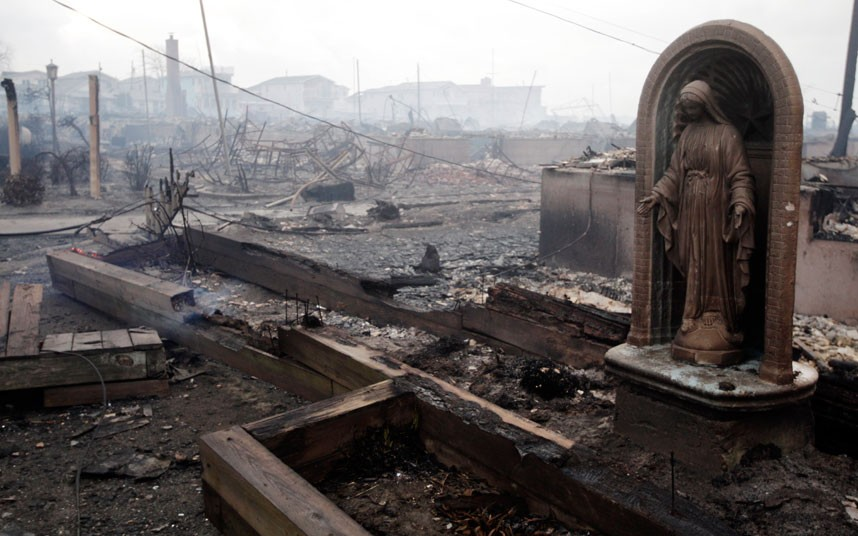
\includegraphics[width=\linewidth]{images/real_example.jpg}
        \caption{Recovering From Sandy: Breezy Point, Queens; Santiago, Cuba}
        \label{fig:real}
    \end{subfigure}
    \hfill % separation between the subfigures
    \begin{subfigure}[b]{0.3\textwidth}
        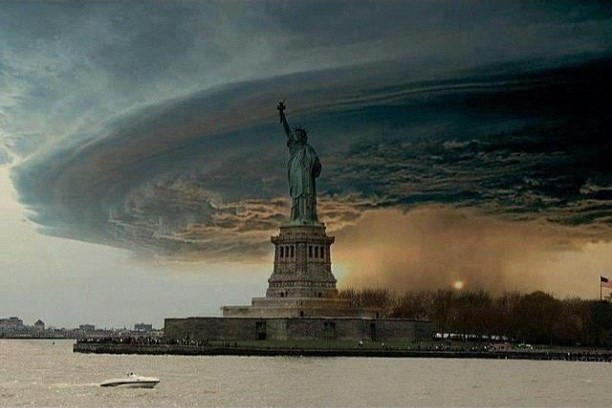
\includegraphics[width=\linewidth]{images/fake_example.jpg}
        \caption{New York gonna be screwed \#sandy \#hurricane \#newyork \#fucked}
        \label{fig:fake}
    \end{subfigure}
    \hfill % separation between the subfigures
    \begin{subfigure}[b]{0.3\textwidth}
        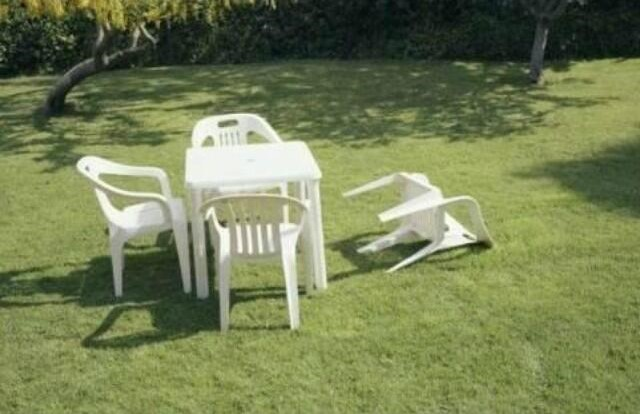
\includegraphics[width=\linewidth]{images/humor_example.jpg}
        \caption{Britain's last hurricane was devastating...}
        \label{fig:humor}
    \end{subfigure}
    \caption{当研究で扱う3カテゴリの投稿例: (a)正しいニュース,(b)フェイクニュース,(c)ジョークニュース}
    \label{fig:examples}
\end{figure}

いずれも2012年に発生したハリケーン・サンディに関してTwitter上で投稿されたものであった.
図\ref{fig:real}は実際に撮影された被害を免れた聖母マリア像を写したもの,
図\ref{fig:fake}は2004年に撮影された写真に自由の女神を合成させたもの\cite{harmanci_2012},
図\ref{fig:humor}はイギリスにハリケーンが来ないことを茶化すものである.

%
当研究では,上記対象を正確に3カテゴリへ分類するモデルを構築することを目標としている.
具体的には,入力として画像と文章を持ち,それに対してどのカテゴリが該当するかを出力するモデルとなる.

当研究を更に発展させると,SNS上でユーザや運営側を支援するエージェント開発に繋げることができる.
%
%
\chapter{提案手法}
%
\section{エージェント詳細}
% 
本章では韻律的特徴量から発話者の感情を推定するシステム,及び,それを使用した
応答変更機能のある対話エージェントの提案を行う.提案手法のエージェントの応答の流れを図\ref{fig:system_pic31}に示す.

\begin{figure}[h]
	\centering
		\fbox{\includegraphics[width=\fullwidth]{./img/agent.png}}
        \caption{提案手法のエージェントの応答の流れ}
        \label{fig:system_pic31}
	\centering
\end{figure}

ユーザは初めにエージェントに向かって音声を入力する.その後エージェントは入力された音声から韻律的特徴量を抽出し,識別機にその特徴量を入力する.識別機はその特徴量から話者の感情を推定し,その推定底結果からエージェントは応答を生成し,音声として出力する.
%
%
\section{韻律情報}
韻律情報とは音声の高さや大きさ,速さ,長さ,イントネーション等,文字に現れない話者の発話の特徴である.これらの情報は個人により異なり,また一人ひとりの発話の方法でも差異が生じてくる.この差異を数としてとらえるために使用するものが韻律的特徴量であり,後述する感情推定システムで使用される.

\section{韻律的特徴量を用いた感情推定システム}
%
\subsection{韻律的特徴量}
韻律的特徴量とはパワーやピッチといった音声に関する特徴量のことを指す.
本システムで使用する韻律的特徴量はINTERSPEECH 2009 Emotion Challenge\cite{tokutyou}で使用された特徴量を用いた.表\ref{tokutyou}に一覧を示す.

\begin{table}[h]
\begin{center}
%韻律的特徴量
	\caption{韻律的特徴量}
	\begin{tabular}{c|c|c} \hline
		特徴量名 & $\Delta$成分 & 統計量(12種) \\ \hline \hline
		RMS energy & $\Delta$ RMS energy & amean \\ \cline{1-2}%1
		F0 & $\Delta$ F0 \hline & standard deviation \\ \cline{1-2}%2
		ZCR & $\Delta$ ZCR \hline & max, maxPos, min, minPos \\ \cline{1-2}
		voice Prob & $\Delta$ voice Prob \hline  & range, skewness, kurtosis \\ \cline{1-2}
		MFCC 1-12 & $\Delta$ MFCC 1-12 \hline & linregc 1, linregc 2, linregerrQ \\ \hline%3
	\end{tabular}
	\label{tokutyou}
\end{center}
\end{table}

特徴量の具体的な内容は,各フレームごとの平均パワー,ピッチ周波数,ゼロ交差率,Voice probability(全パワーに占める調波成分の割合),
12次元のMFCCの計16次元とその{\Delta}成分が16次元,
さらにその32次元に対し12種類の統計量(平均,標準誤差,最大値とその位置,最小値とその位置,値のレンジ,尖度,歪度,
1次の回帰係数とその切片,回帰誤差)をとった32*12=384次元である.
%+特徴量説明

韻律的特徴量の抽出にはオープンソフトウェアのであるOpenSMILE\cite{opensmile}を使用した.OpenSMILEはミュンヘン工科大学が開発した,「音声認識」,「音楽認識」,「パラ言語認識」等の研究向けに作られた音声特徴量抽出ソフトウェアである.

%
%\newpage
%
\subsection{識別機の作成}
識別機は入力を発話の韻律的特徴量,出力を発話者の感情値とする.
識別機の作成にはオープンソースの機械学習ソフトウェアであるWeka\cite{weka}のSupport Vector Regression(SVR)を用いた.
%+SVRの説明
また学習用の対話コーパスは宇都宮大学パラ言語情報研究向け音声対話データベース\cite{taiwa}を使用した.
このデータベースは親しい間柄の6ペアの発話内容が記録されており,全部で4840発話が収録されている.
発話には快-不快,覚醒-睡眠,支配-服従,信頼‐不信,関心‐無関心,肯定的,否定的の6感情についてラベルが付与されている.

識別機の作成は,学習用対話コーパスの発話群の韻律的特徴量を抽出し,それを付与されている6感情それぞれについてSVRによって学習させることで作成した.

\section{感情に応じた応答生成}
識別機によって出力された感情値を用いて応答の変更を行う.
ある感情の推測値に対して閾値を設ける.それぞれの感情の推測値がその閾値を上回るかどうかを判定し,上回った感情の組み合わせによって応答を変更し生成する.
これにより,文字等の言語情報を用いずに応答を変更することができる.

%図の挿入


%
%
\newpage
%
%
%
%
%
%
%
%
%
%
% 
%
\chapter{評価実験}
%
\section{データセット}
% 
\section{比較対象手法}
% 
\section{実験条件}
% 
\section{実験結果}
% 

\chapter{評価}

\section{考察}

\section{課題}


%
%
\chapter{おわりに}
%
\section{本論文のまとめ}
%
\section{今後の展望}
% 

%謝辞
\chapter*{謝辞}
\addcontentsline{toc}{chapter}{謝辞}
本研究を行うにあたり,ご多忙の中,終始適切かつ丁寧なご指導をして下さった大須賀昭彦教授,田原康之准教授,清雄一准教授に深く感謝致します.貴重な勉学の機会を与えてくださったことに深く御礼申し上げます.

%また,研究の機会と議論・研鑽の場を提供して頂き,ご指導頂いた国立情報学研究所/東京大学の本位田真一教授をはじめ活発な議論と貴重なご意見を頂いた研究グループの皆様,大須賀・田原研究室の皆様に感謝の意を表します.さらに,本研究を行う上で必要な楽天公開データの提供に協力してくださいました国立情報学研究所,楽天株式会社の関係者の皆様に感謝の意を表します.

%\chapter*{研究業績}
%\addcontentsline{toc}{chapter}{研究業績}

%\section*{国際会議}
%\begin{achievement}
%\item \underline{\textbf{Minato Sato}}, Ryohei Orihara, Sei Yuichi, Yasuyuki Tahara and Akihiko Ohsuga: Japanese Text Classification by Character-Level Deep ConvNets and Transfer Learning, The 9th International Coneference on Agents and Artificial Intelligence (ICAART2017), Feb 2017. (accepted as a Full Paper)
%\end{achievement}

%\section*{査読付き国内シンポジウム・ワークショップ}
%\begin{achievement}
%\item \underline{\textbf{佐藤挙斗}},折原良平,清雄一,田原康之,大須賀昭彦: 文字レベル深層学習による日本語テキストの分類と転移学習,合同エージェントワークショップ&シンポジウム2016 (JAWS2016),pp.199-206,2016年9月. (ショート発表) \textcolor{red}{{\bf 優秀発表賞}}
%\end{achievement}

%\section*{研究会}
%\begin{achievement}
%\item \underline{\textbf{佐藤挙斗}},折原良平,清雄一,田原康之,大須賀昭彦: 文字レベル深層学習の日本語データセットへの応用,第184回 情報処理学会 知能システム研究会 (SIG-ICS) ,2016年8月.
%\item \underline{\textbf{佐藤挙斗}},折原良平,清雄一,田原康之,大須賀昭彦: 文字レベル深層学習によるテキスト分類と転移学習,人工知能学会 第102回人工知能基本問題研究会(SIG-FPAI),2016年12月. 
%\end{achievement}

%参考文献
\newpage
\printbibliography[title=参考文献]
%付録
%%
\appendix
\renewcommand{\thesection}{付録.\ \arabic{section}}
\renewcommand{\thesubsection}{\ \arabic{section}-\arabic{subsection}}
%
\section{統計表3  推計患者数,年齢階級・傷病大分類別}
\subsection{分類表1}
%
\begin{figure}[h]
  \begin{center}
    \includegraphics[width=\fullwidth]{./img/図1.jpg}
    %\caption{傷病大分類1}
  \end{center}
\end{figure}
%
\newpage
\subsection{分類表2}
%
\begin{figure}[h]
  \begin{center}
    \includegraphics[width=\fullwidth]{./img/図2.jpg}
    %\caption{傷病大分類2}
  \end{center}
\end{figure}
%
\newpage
\section{統計表9  総患者数,性・主な傷病別 }
%
\begin{figure}[h]
  \begin{center}
    \includegraphics[width=0.8\fullwidth]{./img/図3.jpg}
    %\caption{傷病大分類3}
  \end{center}
\end{figure}


%
%
%
\end{document}